\section{Navigation}
Die Navigation in der App lässt sich durch eine gute Domainanalyse vorbereiten. Mit dieser können die Screens entwickelt werden, die es braucht um mit den Daten umgehen zu können.\\
Danach kann man Screens gruppieren. Dies hilft das Design an grosse und kleine Bildschirme anzupassen (siehe Reflow-Pattern, WED2). Danach kann man die Beziehung zwischen den Screens festlegen. Es gibt die \textbf{Parent-Child} Hierarchie, und die \textbf{Siblings}.
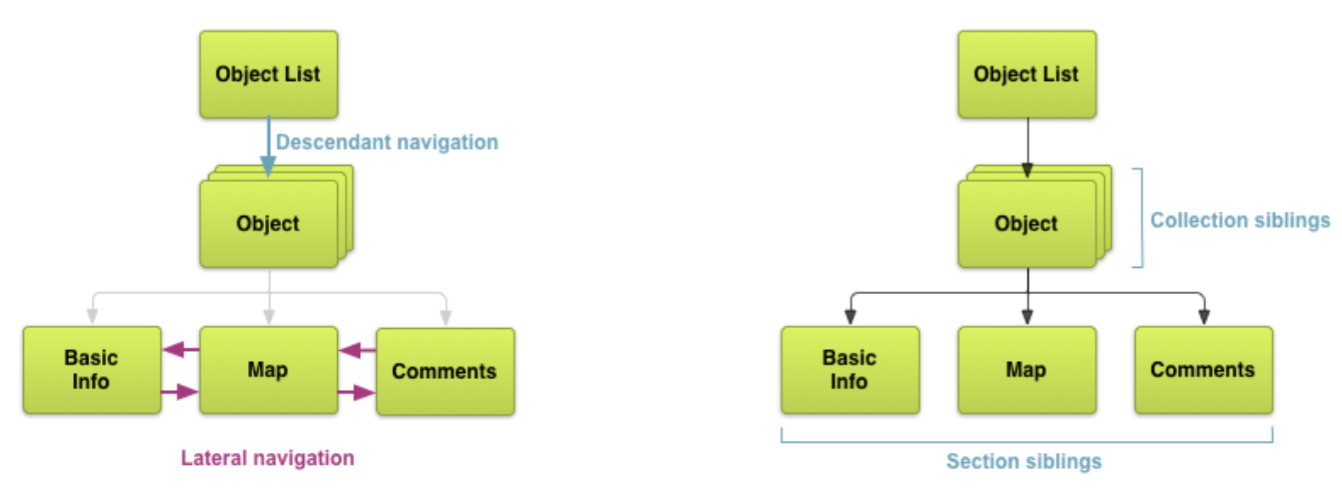
\includegraphics[scale=0.25]{NavScreen.png} \\
Bei der Rückwärtsbeziehung unterscheidet man ebenfalls zwischen 2 Navigationstypen. Die \textbf{Ancestral Navigation} führt zum hierarchischen Parent, die \textbf{Temporal Navigation} führt zum vorherigen Element. Ancestral Navigation geschieht über den Up oder Home Button, Temporal Naviagtion über den Back-Button.\\
Grundsätzlich geht man beim Navigation-Design folgendermassen vor:
\begin{enumerate}
\item Domain-Modell entwerfen
\item Screens ableiten
\item Screens in Beziehung bringen und gruppieren
\item Navigation zwischen den Screens festlegen
\item Wireframe/Storyboard für die Gesamtübersicht erstellen
\item Usability Test mit einem Papier-Prototypen des Wireframes
\end{enumerate}
\paragraph{Fragment} Es ist nicht möglich mehrere Activities auf einem Screen anzuzeigen. Mit Fragments ist das möglich. Ein Fragment ist ein modularer Teil einer Activity mit eigenem Lebenszyklus.
\begin{lstlisting}[language=java]
public class MainActivityFragment extends Fragment {
  public MainActivityFragment() {}
  @Override
  public View onCreateView(LayoutInflater inflater, ViewGroup container, Bundle savedInstanceState) {
  View layout = inflater.inflate(R.layout.fragment_main, container, false);
  counter = (TextView) layout.findViewById(R.id.counter);
  button = layout.findViewById(R.id.button);
  return layout;
  }
}
\end{lstlisting}
Ein Fragment kann im XML in eine Activity eingefügt werden.
\begin{lstlisting}[language=xml]
<?xml version="1.0" encoding="utf-8"?>
<LinearLayout xmlns:android="http://schemas.android.com/apk/res/android"
  android:layout_width="match_parent"
  android:layout_height="match_parent"
  android:orientation="horizontal">
  <fragment xmlns:android="http://schemas.android.com/apk/res/android"
  xmlns:tools="http://schemas.android.com/tools"
  android:id="@+id/fragment"
  android:name="com.example.myfragmentapplication.MainActivityFragment"
  android:layout_width="match_parent"
  android:layout_height="match_parent"
  tools:layout="@layout/fragment_main" />
</LinearLayout>
\end{lstlisting}
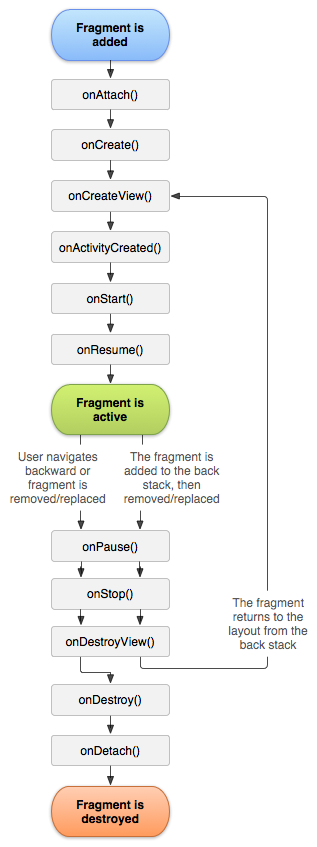
\includegraphics[scale=0.5]{fragment_lifecycle.png}
%TODO: Floating image
Ein Fragment wird einem \code{LayoutInflater} übergeben, der nimmt XML entgegen und instanziert die View Klassen.
Oder dynamisch, mit dem FragmentManager im Java Code
\begin{lstlisting}[language=java]
public class MainActivity extends Activity {
  @Override
  protected void onCreate(Bundle savedInstanceState) {
  super.onCreate(savedInstanceState);
  setContentView(R.layout.activity_main);
  FragmentManager fm = getFragementManager();
  FragmentTransaction ft = fm.beginTransaction();
  MainActivityFragment f = new MainActivityFragment();
  ft.add(R.id.fragment_container, f);
  ft.commit();
  }
...
}
\end{lstlisting}
Best Practice ist, dass Fragments ein Interface zur Kommunikation definieren, welches Parent-Activity implementieren muss.
\begin{lstlisting}[language=java]
public class MainActivityFragment extends Fragement {
  public interface OnItemSelectedlistener {
  void onItemSelected(String item);
  }
  OnItemSelectedListener parentActivity;
  @Override
  public void onAttach(Activity activity) {
  super.onAttach(activity);
  if (!(activity instanceof OnItemSelectedlistener)) throw new AssertionError( "Activity must implement OnItemSelectedlistener!");
  parent = (OnItemSelectedlistener) activity;
  }
}
\end{lstlisting}
\paragraph{Master-Detail Navigation} Die Unterscheidung zwischen den Anzeigevarianten wird über Layouts getroffen. Das Default-Layout der \code{ItemListActivity} beinhaltet nur das \code{ItemListFragment}. Das Tablet enthält ein Linear-Layout mit dem \code{ItemListFragment} sowie ein Platzhalter für das \code{ItemDetailFragment}. Das Kriterium für das Tablet-Layout ist \textit{sw600dp}(smallest width 600dp).
\begin{lstlisting}[language=java]
public clas ItemListActivity extends Activity implements ItemListFragment.Callbacks {
  private boolean twoPane;
  @Override
  protected void onCreate(Bundle savedInstanceState) {
  super.onCreate(savedInstanceState);
  setContentView(R.layout.activity_item_list);
  if(findViewById(R.id.item_details_container) != null) {
    twoPane = true;
  }
  }
  @Override
  public void onItemSelected(String id) {
  if(twoPane) {
    Bundle arguments = new Bundle();
    arguments.putString(ItemDetailFragment.ARG_ITEM_ID, id);
    ItemDetailFragment fragment = new ItemDetailFragment();
    fragment.setArguments(arguments);
    getFragmentManager()
    .beginTransaction()
    .replace(R.di.item_detail_container, fragment)
    .commit();
  } else {
    Intent detailIntent = new Intent(this, ItemDetailActivity.class);
    detailIntent.putExtra(ItemDetailFragment.ARG_ITEM_ID, id);
    startActivity(detailIntent);
  }
  }
}
\end{lstlisting}
Activities sollte man verwenden, wenn man einen Einstiegspunkt in einen Task braucht. \textbf{Wichtig:} Activities leben weiter, wenn wir eine neue Activity starten.

Neben \code{fragmentTransation.add} gibt es noch \code{fragmentTransaction.replace}. Es kann auch direkt \code{replace} aufgerufen werden, auch wenn noch keines ge-addet wurde. Beispiel siehe Spick ''Settings Page''.

\subsection{Activity-Layout für dynamisch}
Frame Layout ''hat sich so eingebürgert''.
\begin{lstlisting}[language=xml]
<LinearLayout>
  <FrameLayout android:id="@+id/fragment_container"/>
</LinearLayout>
\end{lstlisting}

\paragraph{Callback}
Damit Fragments mit der Activity kommunizieren können:
\begin{enumerate}
  \item Interface definieren. Am besten ''event-mässig'', also \code{onEVENT}
  \item Interface auf Activity implementieren
  \item in Fragment im \code{onAttach}:\\ \code{if !(activity instanceof INTERFACE) throw new AssertionError}
\end{enumerate}

\subsection{Verschachtelung}
Ab Android 4.2, API-Level 17, können Fragments verschachtelt werden. Dann muss man mit dem \code{getChildFragmentManager} gearbeitet werden, z.B. beim ViewPager.

\subsection{Backbutton}
\begin{lstlisting}[language=java]
// vorher/nachher:
.replace().commit();
.replace().addToBackStack(null).commit();

public void onBackPressed()  {
  if (getFragmentManager().getBackStackEntryCount() <= 1) { 
  finish();
  } else {
  pages.pop();
  getFragmentManager().popBackStack();
  }
}
\end{lstlisting}

\subsection{Menus}
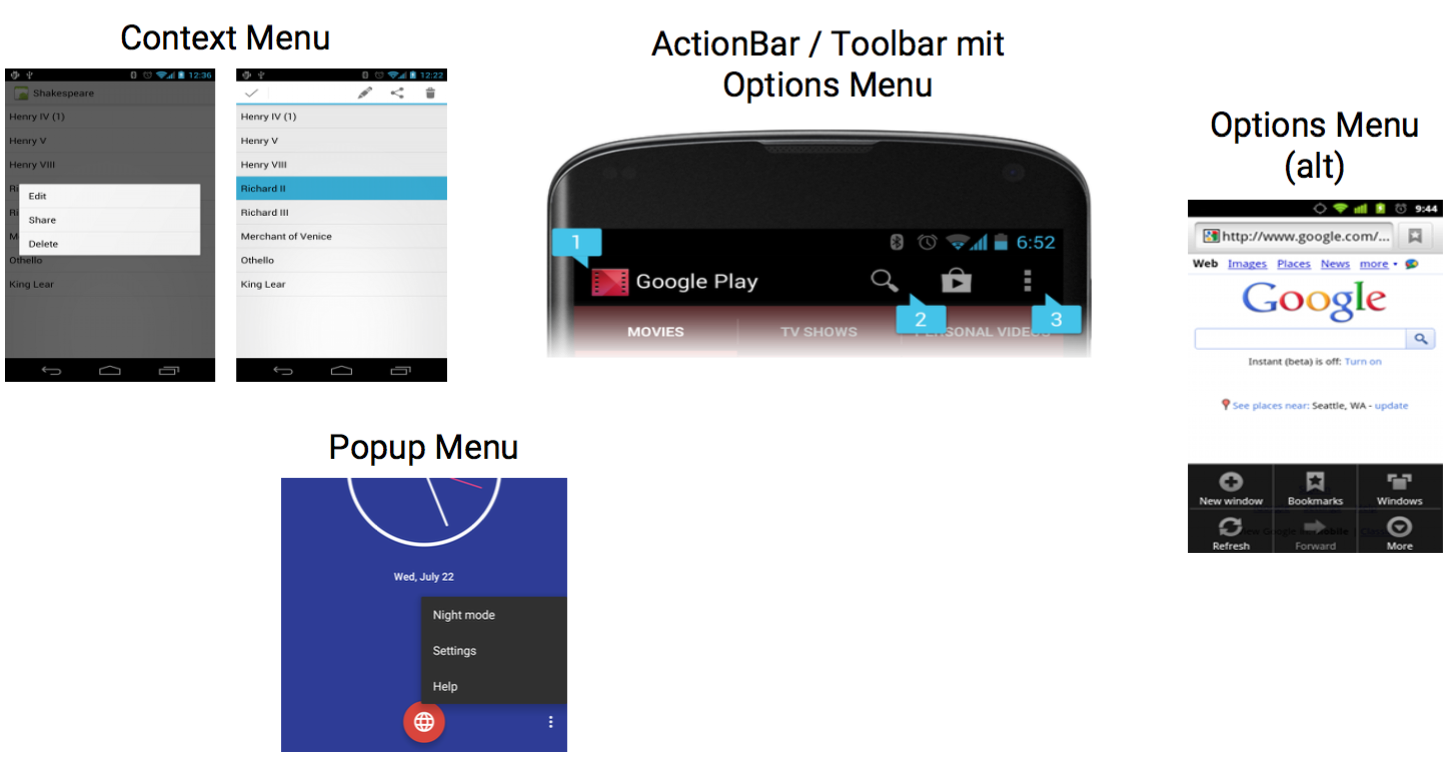
\includegraphics[scale=0.25]{Menus.png}
\paragraph{Options Menu} Das Options Menu ist teil der ActionBar. Es enthält Actions die generell für die App/Activity gedacht sind. Apps mit Navigation Drawer haben teilweise kein Options Menu mehr. \\
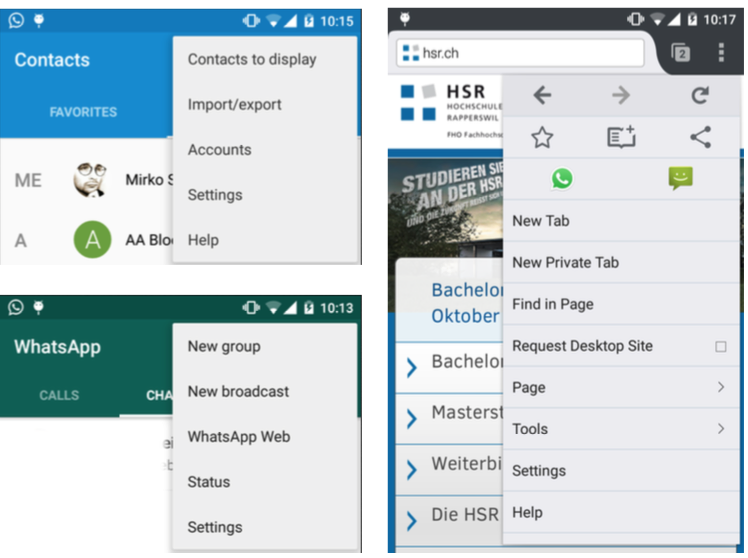
\includegraphics[scale=0.25]{OptionsMenu.png}
\begin{lstlisting}[language=java]
public boolean onCreateOptionsMenu(Menu menu) {
  menu.add(0, START_MENU_ITEM, 0, "Start");
  menu.add(0, SUBMIT_MENU_ITEM, 0, "Submit");
  return true;
}
public boolean onOptionsItemSelected(MenuItem item){
  switch(item.getItemId()){
  case START_MENU_ITEM:
    // start
    return true;
  case SUBMIT_MENU_ITEM:
    // submit
    return true;
  }
  return super.onOptionsItemSelected(item);
}
\end{lstlisting}
Der bessere Ansatz wäre die deklarative Implementation im XML.
\begin{lstlisting}[language=xml]
<menu xmlns:android="http://schemas.android.com/apk/res/android"
xmlns:tools="http://schemas.android.com/tools" tools:context=".MainActivity">
  <item android:id="@+id/action_search"
  android:title="@string/action_search"
  android:icon="@drawable/ic_action_search"
  android:orderInCategory="100"
  android:showAsAction="never" />
  <item android:id="@+id/action_settings"
  android:title="@string/action_settings"
  android:orderInCategory="100"
  android:showAsAction="never" />
</menu>
\end{lstlisting}
\begin{lstlisting}[language=java]
public class MainActivity extends Activity {
  public boolean onCreateOptionsMenu(Menu menu) {
  getMenuInflater().inflate(R.menu.menu_main, menu);
  return true;
  }
  public boolean onOptionsItemSelected(MenuItem item) {
  /* ... */
  }
}
\end{lstlisting}
\paragraph{Settings-Page} Die Settings-Page erbt von der Klasse \code{PreferenceActivity}. Sie kann im \code{PreferenceScreen} Tag definiert werden.
\begin{lstlisting}[language=xml]
<!-- preferences.xml -->
<PreferenceScreen xmlns:android="...">
  <CheckBoxPreference
  android:defaultValue="true"
  android:key="@string/sync_pref"
  android:title="Synchronize" />
  <MultiSelectListPreference
  android:entries="@array/languages"
  android:entryValues="@array/languages"
  android:key="@string/lang_pref"
  android:title="Languages" />
</PreferenceScreen>
<!-- resources.xml -->
<resources>
  <string name="lang_pref">language</string>
  <string name="sync_pref">synchronize</string>
  <string-array name="languages">
  <item>German (CH)</item>
  <item>English (UK)</item>
  </string-array>
</resources>
\end{lstlisting}
\begin{lstlisting}[language=java]
public class Preferences extends PreferenceActivity {
  @Override
  public void onCreate(Bundle savedInstanceState) {
  super.onCreate(savedInstanceState);
  getFragmentManager()
    .beginTransaction()
    .replace(R.id.content, new PrefsFragment()
    .commit();
  PreferenceManager.setDefaultValues(this, R.xml.preferences, false);
  }
  public static class PrefsFragment extends PreferenceFragment {
  @Override
  public void onCreate(Bundle savedinstanceState) {
    super.onCreate(savedInstanceState);
    addPreferencesFromResource(R.xml.preferences);
  }
  }
}
\end{lstlisting}
In der MainActivity mit dem Settings-Menueintrag brauchen wir bloss noch die neue Activity zu starten.
\begin{lstlisting}[language=java]
@Override
public boolean onOptionsItemSelected(MenuItem item){
  int id = item.getItemId();
  if(id == R.id.action_settings) {
  startActivity(new Intent(this, Prefernces.class));
  return true;
  }
  return super.onOptionSItemSelected(item);
}
\end{lstlisting}
Die Einstellung wird mittels dieser Funktion ausgelesen.
\begin{lstlisting}[language=java]
SharedPreferences settings = getSharedPreferences(FILENAME, 
  MODE_PRIVATE); // alternativ: MODE_MULTI_PROCESS
SharedPreferences.Editor editor = settings.edit();
editor.putBoolean("disabled", false)

boolean isDisabled = settings.getBoolean("disabled", false)
// false ist Defaultwert falls nicht existent

editor.commit();
\end{lstlisting}
Auch Fragments können Einträge dem Menu der Activity hinzufügen. Die Behandlung erfolgt analog entweder im Fragment oder in der Activity.
\begin{lstlisting}[language=java]
public class MainFragment extends Fragment {
  @Override
  public void onCreateOptionsMenu(Menu menu, MenuInflater inflater) {
  inflater.inflate(R.menu.menu_main, menu);
  }
  @Override
  public void onCreate(Bundle savedInstanceState) {
  super.onCreate(savedInstanceState);
  setHasOptionsMenu(true);
  }
}
\end{lstlisting}
\paragraph{Context und Popup Menu} Ein Context Menü für Actions welche die selektierte View betreffen. Meist ändert sich bei einer Selektion die ActionBar.\\
Popup Menüs lassen sich z.B an einen beliebigen Button binden (Vergleichbar mit einem Spinner/Combobox). \\
Popup Menus eignen sich für Overflow-Style Menu für Actions die Context spezifisch sind (beispielsweise Weiterleiten und Antworten bei Mail). 
\begin{lstlisting}[language=xml]
<ImageButton
  android:layout_width="wrap_content" 
  android:layout_height="wrap_content" 
  android:src="@drawable/ic_overflow_holo_dark"
  android:contentDescription="@string/descr_overflow_button"
  android:onClick="showPopup" />
\end{lstlisting}
\begin{lstlisting}[language=java]
public void showPopup(View v) {
  PopupMenu popup = new PopupMenu(this, v);
  MenuInflater inflater = popup.getMenuInflater();
  inflater.inflate(R.menu.actions, popup.getMenu());
  popup.show();
}
\end{lstlisting}
\paragraph{Action Bar} Die ActionBar war der erste Versuch eine normierte "{}Schnittstelle"{} für Aktionen in einer App zu kreieren. \\
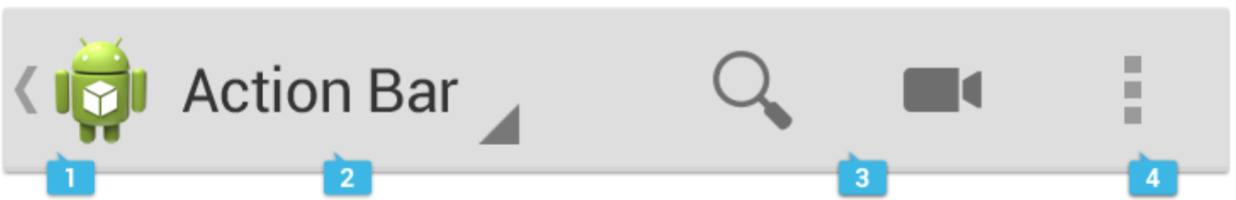
\includegraphics[scale=0.25]{ActionBar.png}
\begin{enumerate}
\item App Icon und ev. Up-/Home-Navigation
\item Name der App oder View-Switcher
\item Actions (Teil des Options Menu)
\item Action-Overflow mit dem Rest des Menus
\end{enumerate}
\paragraph{Toolbar} Die Toolbar soll ab Android 5.0 die ActionBar ablösen. Sie ist flexibler aber noch nicht so weit verbreitet. Um sie in älteren Android Versionen verwenden zu können ist eine Support-Library nötig.

\includegraphics[scale=0.35]{toolbar.png}
\begin{lstlisting}[language=xml]
<RelativeLayout xmlns:android="..." xmlns:app="..." xmlns:tools="..."
  android:layout_width="match_parent" android:layout_height="match_parent"
  tools:context=".MainActivity">
  <android.support.v7.widget.Toolbar
  android:id="@+id/toolbar"
  android:layout_width="match_parent"
  android:layout_height="wrap_content">
  </android.support.v7.widget.Toolbar>
  <fragment
  ...
  android:layout_below="@+id/toolbar"
  tools:layout="@layout/fragment_main" />
</RelativeLayout>
\end{lstlisting}
Damit die Toolbar als ActionBar funktioniert braucht es zusätzliche Konfiguration im Java Code
\begin{lstlisting}[language=java]
public class MainActivity extends AppCompatActivity {
  @Override
  protected void onCreate(Bundle savedInstanceState) {
  super.onCreate(savedInstanceState);
  setContentView(R.layout.activity_main);
  Toolbar toolbar = (Toolbar)findViewById(R.id.toolbar);
  setSupportActionBar(toolbar);
  }
}
\end{lstlisting}
\paragraph{Navigation Drawer} Dies ist eine Art Hauptmenü. Es wechselt zwischen Activities oder Fragments. Es können auch gewisse Einstellungen verändert werden (Toggle). \\
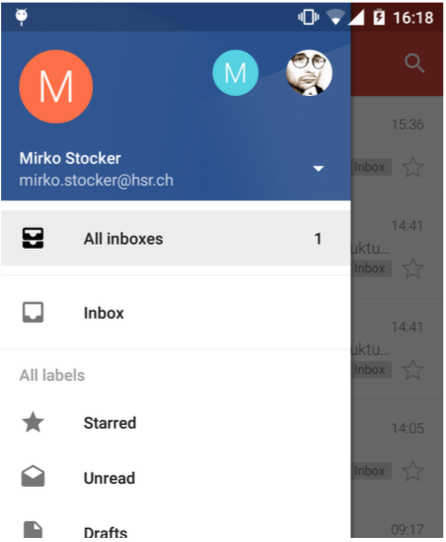
\includegraphics[scale=0.35]{navigationdrawer.png} \\
Der Drawer benötigt eine Layoutdefinition und eine Menudeklaration. Das Layout der Activity ist rechts vom Navigation Drawer und braucht ein FrameLayout.
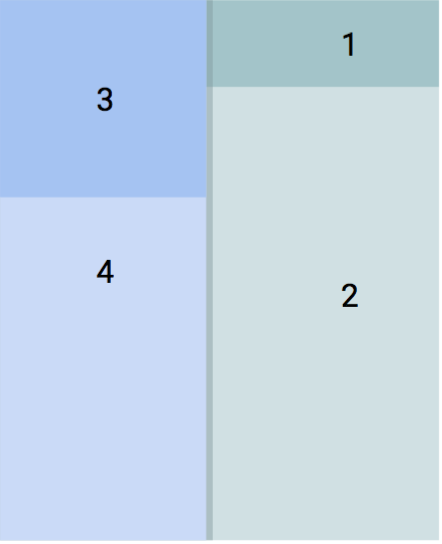
\includegraphics[scale=0.25]{NavDrawer.png}
1. Toolbar, 2. Content, 3. Header, 4. Menu-Items
\begin{lstlisting}[language=xml]
<android.support.v4.widget.DrawerLayout xmlns:android="..." xmlns:app="..." xmlns:tools="..."
  android:id="@+id/drawer_layout"
  android:fitsSystemWindows="true"
  tools:context=".MainActivity">
  <FrameLayout
  android:id="@+id/content"
  android:orientation="vertical">
  <android.support.v7.widget.Toolbar
    android:id="@+id/toolbar"/>
  <TextView ... />
  </FrameLayout>
  <android.support.design.widget.NavigationView
  android:id="@+id/navigation_view"
  android:layout_gravity="start"
  app:headerLayout="@layout/drawer_header"
  app:menu="@menu/drawer" />
</android.support.v4.widget.DrawerLayout>
\end{lstlisting}
In der Activity kann ein Listener registriert werden, welcher auf Menüpunkte des Drawers reagiert.
\begin{lstlisting}[language=java]
NavigationView view = (NavigationView)findViewById(R.id.navigation_view);
view.setNavigationItemSelectedListener(
  new NavigationView.OnNavigationItemSelectedListener() {
  @Override
  public boolean onNavigationItemSelected(MenuItem item) {
  item.setChecked(true);
  drawerLayout.closeDrawers();
  return true;
  }
});
\end{lstlisting}

\paragraph{Menüs}
Im Handler: \code{true} bedeutet ''behandelt''.

Von Fragments aus können auch Menü-Optionen hinzugefügt werden. Dazu gibt es auch dort \code{onCreateOptionsMenu(Menu menu, MenuInflater inflater)}, dort wird der Inflater also bereits mitgegeben.

In \code{onCreate} muss unbedingt \code{setHasOptionsMenusetHasOptionsMenu(true)} gesetzt werden, sonst wird wahrscheinlich das Callback nie aufgerufen
\paragraph{Toast und Snackbar} Toast sind kleine Feedbacknachrichten. Sie werden mit \code{Toast.makeText(...).show()} angezeigt.